\documentclass[11pt]{article}
\usepackage[paperwidth=420mm,paperheight=219mm,margin=13mm]{geometry}
\usepackage[T1]{fontenc}\usepackage{tgpagella,tgheros,tikz,booktabs,tabularx,array}
\usetikzlibrary{arrows.meta,calc}
\pagestyle{empty}\setlength{\parindent}{0pt}
\definecolor{ink}{HTML}{193A40}\definecolor{teal}{HTML}{116754}\definecolor{blue}{HTML}{225C91}
\definecolor{gold}{HTML}{925D20}\definecolor{grey}{HTML}{567374}
\color{ink}\newcommand{\heading}[1]{\par\medskip{\sffamily\large\bfseries #1}\par\smallskip}
\tikzset{job/.style={font=\sffamily,align=center,rounded corners=2pt,minimum width=4.45cm,minimum height=.80cm},
 arr/.style={-{Stealth[length=2mm]},draw=grey}, base/.style={arr,draw=blue},
 dep/.style={arr,draw=gold,dashed},rowname/.style={anchor=west,align=left,font=\sffamily\small}}
\newcommand{\jobnumber}[1]{\ifnum\numexpr#1\relax<10 0\fi\number\numexpr#1\relax}
\begin{document}
{\sffamily\bfseries\color{teal}Local orchestration\hfill Formal training seed 101}\par\medskip
{\LARGE Asynchronous dispatch on one workstation}\par
\heading{Preparation}
\begin{center}
\begin{tikzpicture}
\foreach \x/\id/\label in {0/i/{Inspect six models\\State, actions and parameter counts},9/t/{Tune 24 candidates, 12 at a time\\Four per map and algorithm; 1,000 episodes},18/f/{Freeze six winning configurations\\Use development validation; seed 9001},27/v/{Verify the frozen source and configurations\\Complete the extended runtime checks}}{
\node[job,fill=grey!9,draw=grey!55,minimum width=8.4cm,minimum height=1.15cm] (\id) at (\x,0) {\label};}
\draw[arr] (i)--(t);\draw[arr](t)--(f);\draw[arr](f)--(v);
\end{tikzpicture}\end{center}
\heading{Release jobs independently in each column}
\begin{center}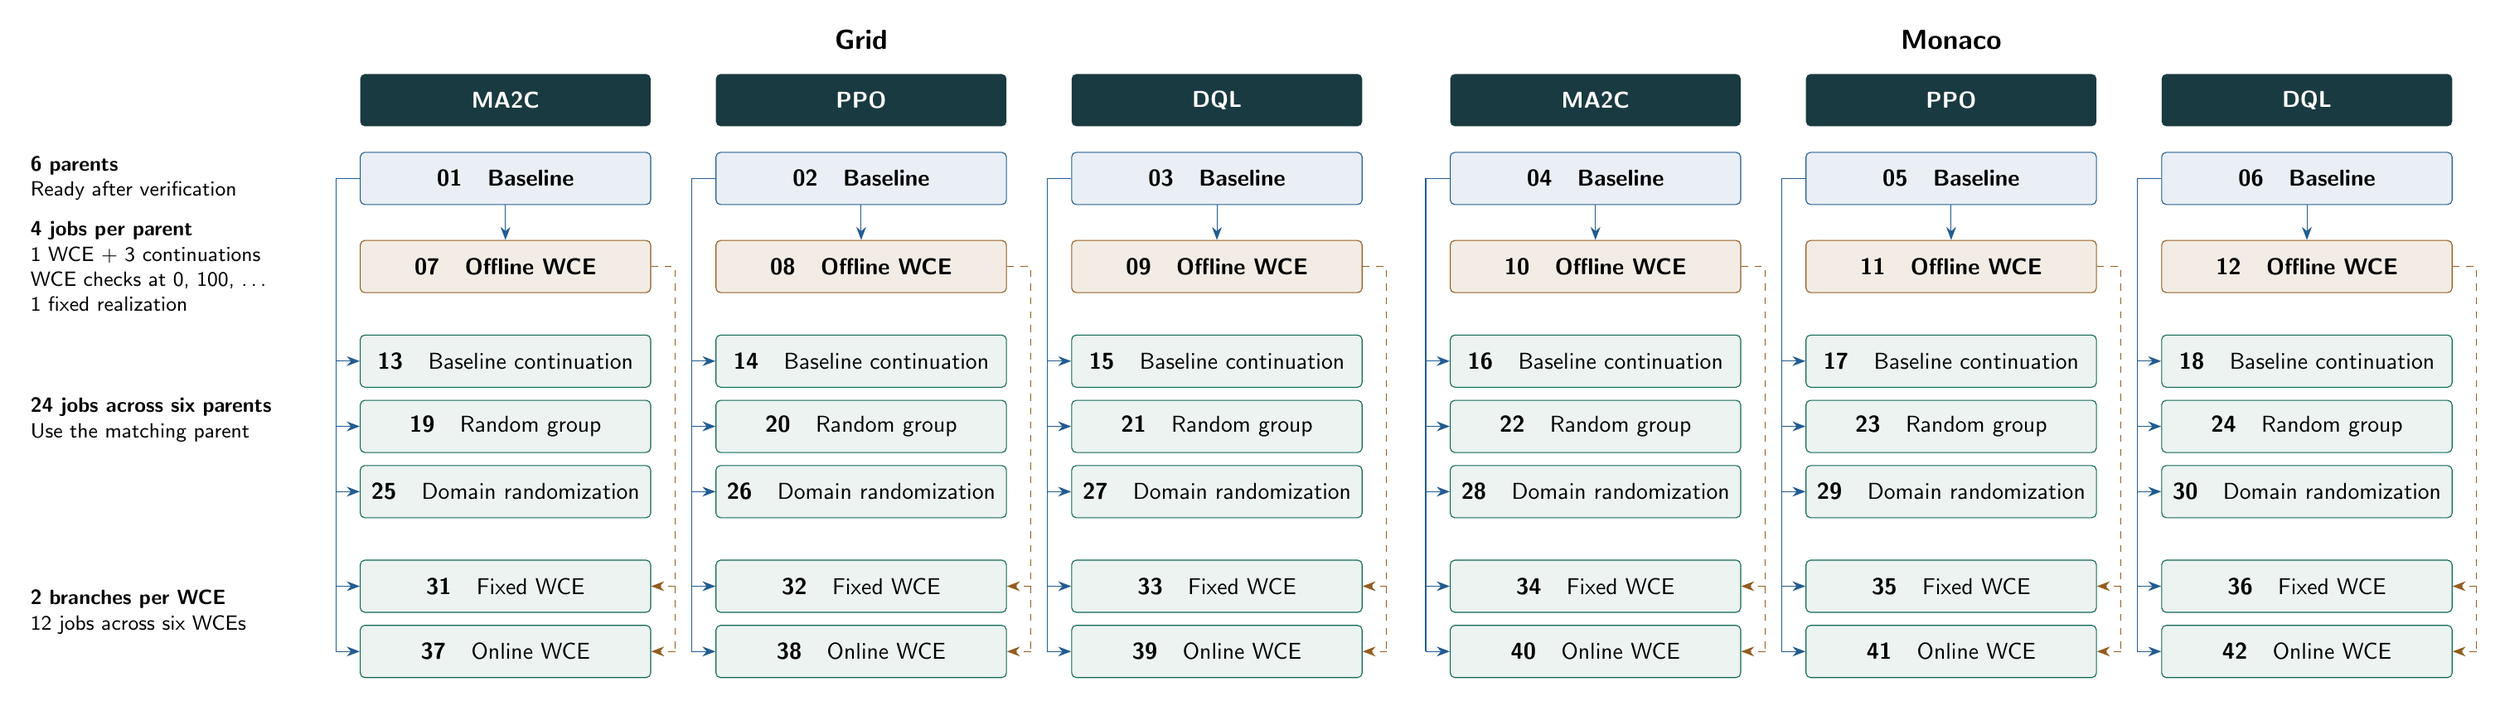
\begin{tikzpicture}
\foreach \x/\n/\alg in {0/1/MA2C,5.45/2/PPO,10.9/3/DQL,16.7/4/MA2C,22.15/5/PPO,27.6/6/DQL}{
\begin{scope}[xshift=\x cm]
\node[job,fill=ink,text=white] at (0,0) {\bfseries\alg};
\node[job,fill=blue!10,draw=blue] (p\n) at (0,-1.2) {\bfseries\jobnumber{\n}\quad Baseline};
\node[job,fill=gold!12,draw=gold] (w\n) at (0,-2.55) {\bfseries\jobnumber{\n+6}\quad Offline WCE};
\draw[base] (p\n)--(w\n);
\draw[blue] (p\n.west)--(-2.6,-1.2)--(-2.6,-8.45);
\foreach \y/\offset/\name in {-4/12/Baseline continuation,-5/18/Random group,-6/24/Domain randomization,-7.45/30/Fixed WCE,-8.45/36/Online WCE}{
\node[job,fill=teal!8,draw=teal] (b\n-\offset) at (0,\y) {\bfseries\jobnumber{\n+\offset}\quad\normalfont\sffamily\name};
\draw[base](-2.6,\y)--(b\n-\offset.west);}
\draw[gold,dashed] (w\n.east)--(2.60,-2.55)--(2.60,-8.45);
\foreach \y/\off in {-7.45/30,-8.45/36}{\draw[dep](2.6,\y)--(b\n-\off.east);}
\end{scope}}
\node[font=\sffamily\bfseries\large] at (5.45,.92){Grid};
\node[font=\sffamily\bfseries\large] at (22.15,.92){Monaco};
\node[rowname] at (-7.4,-1.2){\textbf{6 parents}\\Ready after verification};
\node[rowname] at (-7.4,-2.55){\textbf{4 jobs per parent}\\1 WCE + 3 continuations\\WCE checks at 0, 100, \ldots{}\\1 fixed realization};
\node[rowname] at (-7.4,-4.9){\textbf{24 jobs across six parents}\\Use the matching parent};
\node[rowname] at (-7.4,-7.85){\textbf{2 branches per WCE}\\12 jobs across six WCEs};
\end{tikzpicture}\end{center}
\begin{minipage}[t]{.47\linewidth}
\heading{One pool for training and evaluation}
This host exposes 20 cores and 20 hardware threads. The default pool reserves four cores and budgets 16. With 24 ready one-core jobs and sufficient RAM and disk, 16 run and eight wait. Tuning uses 12 single-core slots. Resource measurements run alongside training. Every five seconds, free slots go to ready jobs that fit.
\end{minipage}\hfill\begin{minipage}[t]{.49\linewidth}
\heading{From each continuation to the paired report}
Each finished branch releases 23 scenario jobs for its best controller through stopping. Each scenario runs ten realizations. The report aggregates all 6,900 rollouts. The local dashboard shows dependencies, progress, training and validation rewards, mean queues and resource waits; operators can release, pause and resume work.
\end{minipage}
\medskip\hrule\medskip
{\sffamily\small\textbf{Example}\quad 01 releases 07, 13, 19 and 25. When 07 finishes, 31 and 37 can start even while 13 or a parent in another column is still running. Solid blue arrows carry the best parent; dashed amber arrows carry the best WCE.}
\end{document}
